	\documentclass{article}
\usepackage[utf8]{inputenc}
\usepackage{graphicx}
\usepackage[margin=2.5cm]{geometry}
\usepackage{eso-pic}
\usepackage{hyperref}
\usepackage{wrapfig}
\usepackage{lipsum}
\usepackage{array}
\usepackage{enumitem}
\AddToShipoutPictureBG{%
    \AtPageLowerLeft{
        % \hspace{1cm}
        
\includegraphics[width=4.5cm]{img/Java-Hutts2.png}
    }
}
\title{Architectural Design Specification}
\date{2017}
\def \project{Electronic ID Verification }
\begin{document}

\makeatletter
    \begin{titlepage}
        \begin{center}
            
\includegraphics[width=0.7\linewidth]{img/up.png}\\[4ex]
            {\huge \bfseries \@title }\\[2ex]
            {\LARGE \textbf{Team:} Java the Hutts}\\[2ex]
            {\LARGE \@date}\\[2ex]
            {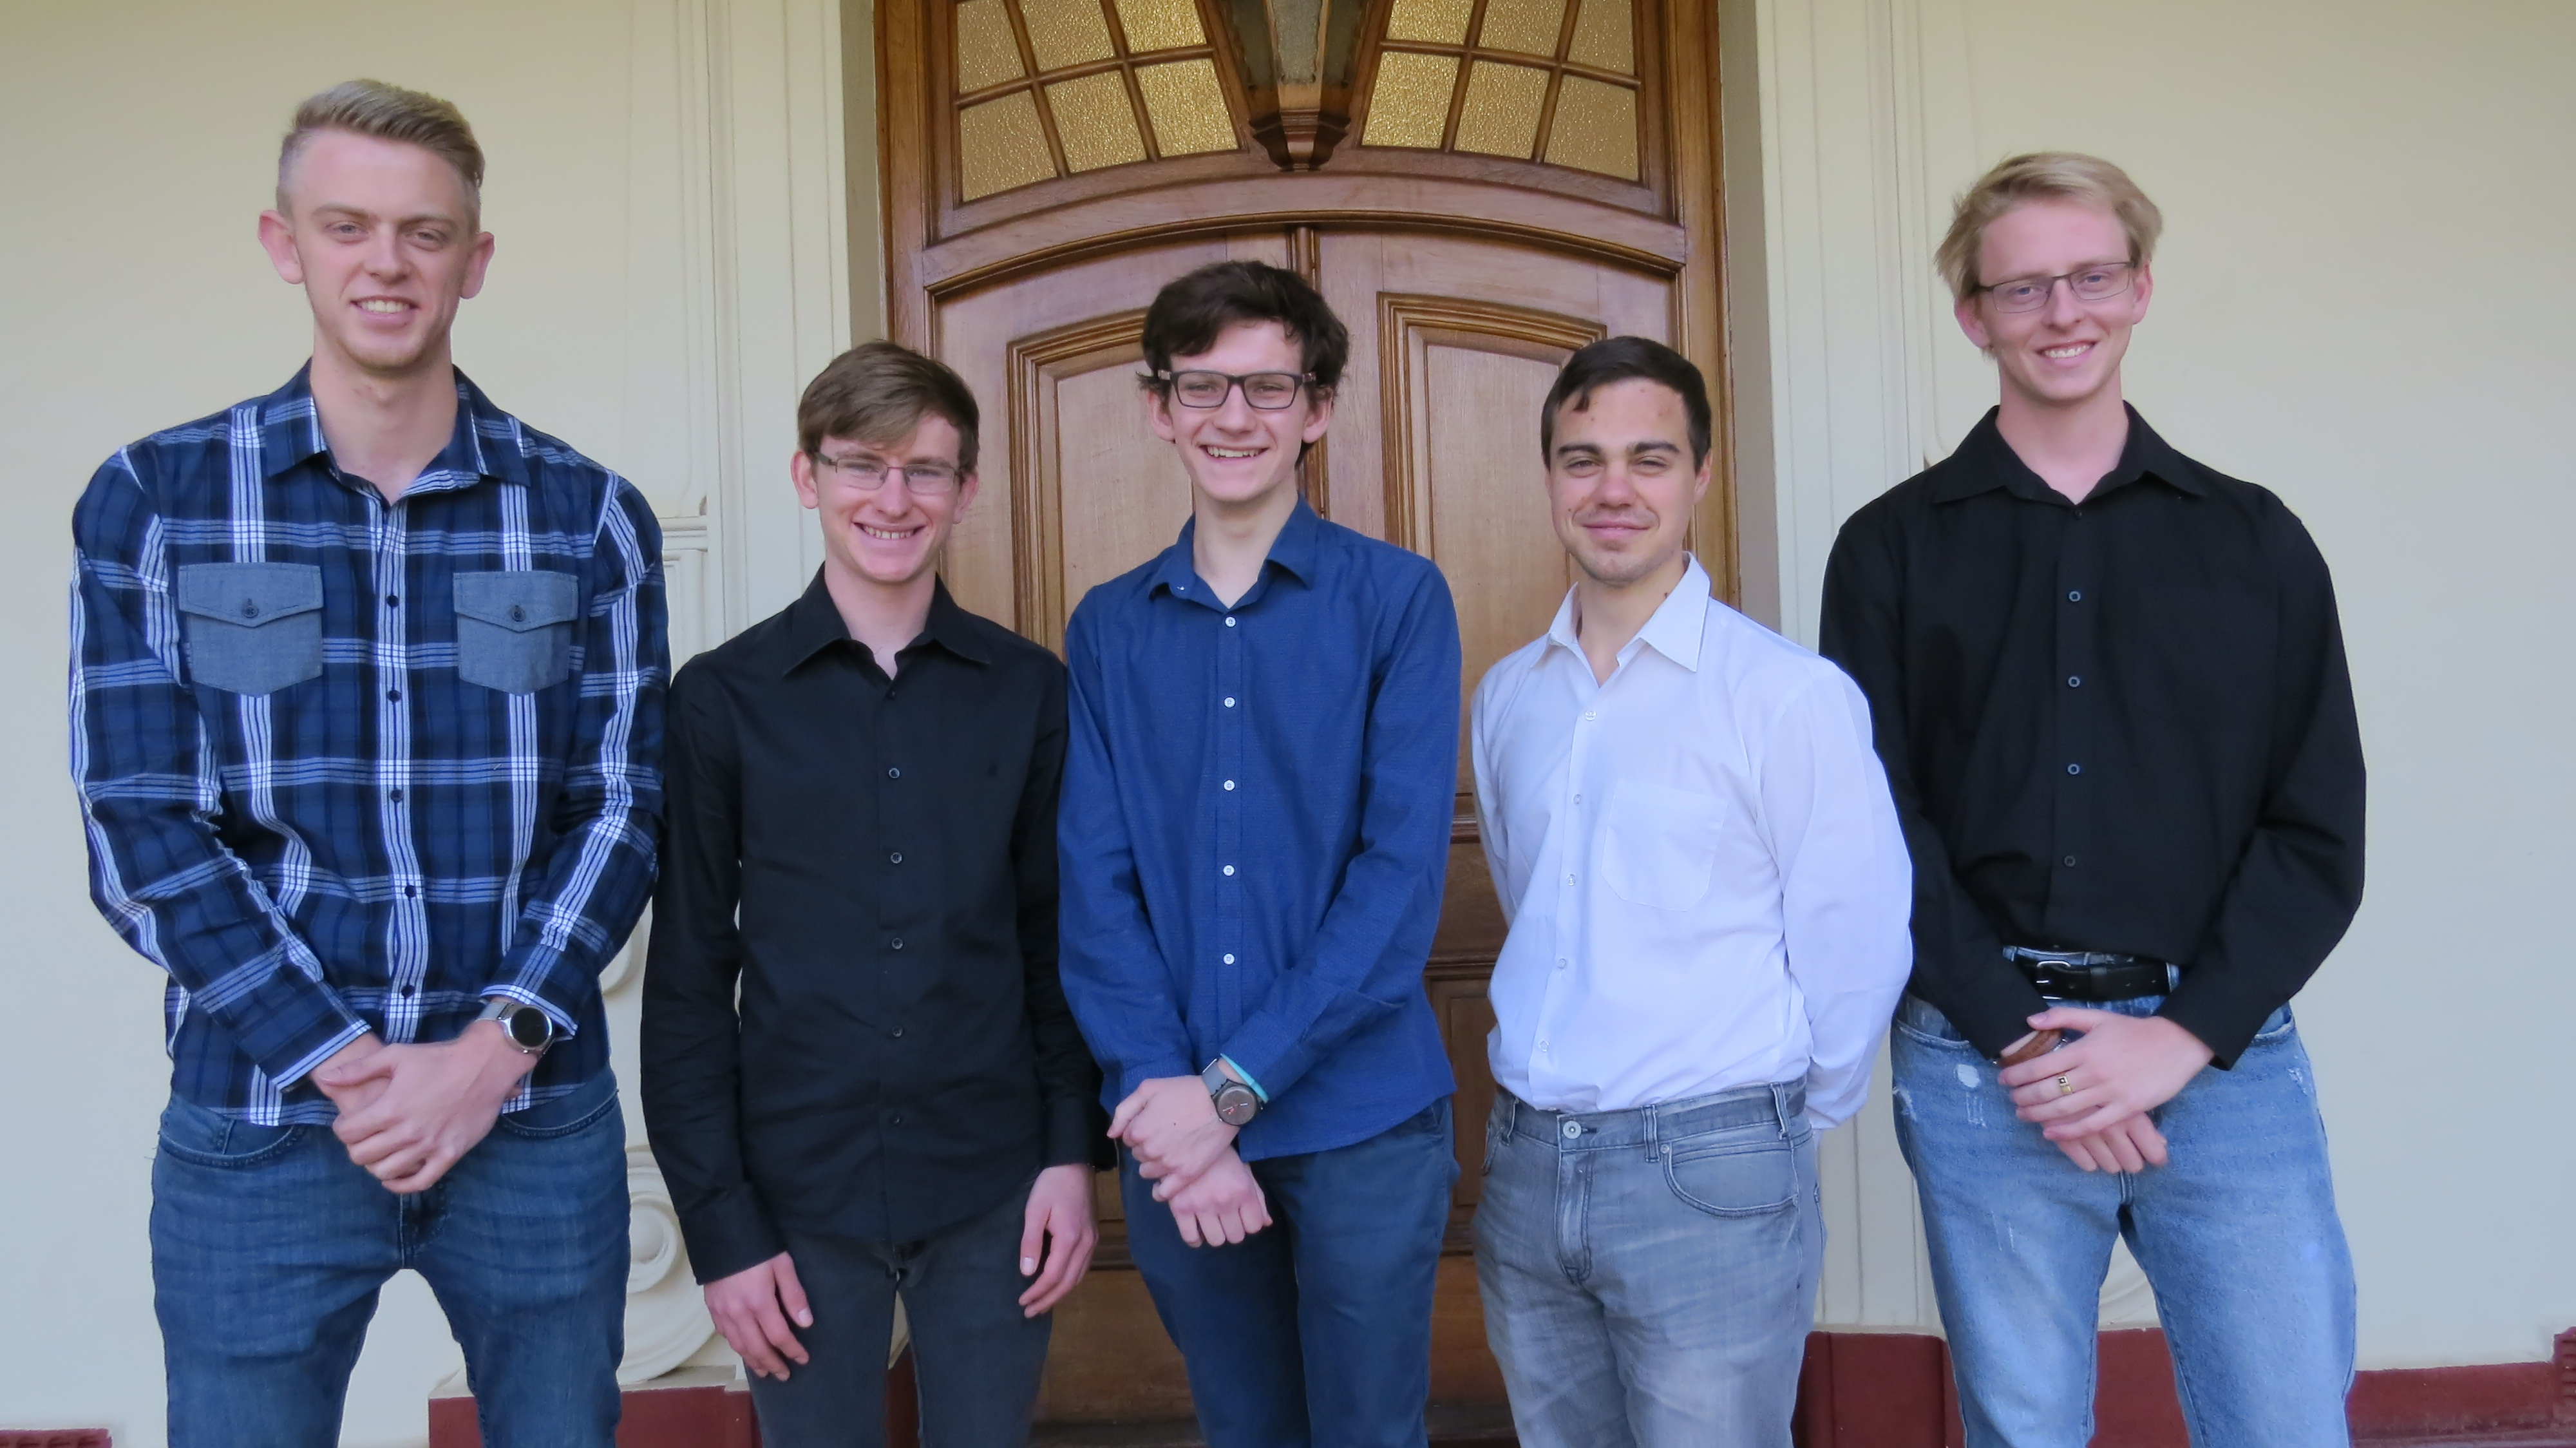
\includegraphics[width=\linewidth]{img/team_photo.jpg}}\\[2ex]
            {\large  Nicolai van Niekerk\\ \texttt{nicvaniek@gmail.com}}\\[2ex]
            {\large  Marno Hermann\\ \texttt{marno@barnton-consulting.co.za}}\\[2ex]
            {\large  Stephan Nell\\ \texttt{nellstephanj@gmail.com}}\\[2ex]
            {\large  Jan-Justin van Tonder\\ \texttt{J.vanTonder@tuks.co.za}}\\[2ex]
            {\large  Andreas Nel\\ \texttt{nel.andreas1@gmail.com}}\\[2ex]
        \end{center}
        
    \end{titlepage}
\makeatother

\cleardoublepage
\thispagestyle{empty}
\tableofcontents
\newpage

\setcounter{page}{1}
	\section{Introduction}
	\subsection{Overview}
This document identifies the architectural design specifications that satisfy the functional requirements proposed in the System Requirements Specification. It addresses the needs of the various subsystems' non-functional requirements focusing on the quality attributes, architectural patterns as well as constraints and integration requirements of the Hutts-Verification system.\newline \newline 
The following modules' designs are included in this document:
\begin{itemize}
	\item Image Processing
	\item Extraction
	\item Verification
\end{itemize}
The document begins with an explanation on the chosen architectural pattern and how it will be used to modularize the API. It then outlines the architectural design of each module along with all relevant UML diagrams. Finally the chosen technologies are discussed as well as the deployment of the system. 

\subsection{Architectural Pattern}
The Hutts-Validation system will be designed as a WebAPI using the Service-Oriented Architecture (SOA). In this pattern, the architecture is essentially a collection of independent services that communicate with each other. Each service is well-defined, self-contained and does not depend on the context or state of other services, ensuring loose coupling. The API will consist of three independent services: Image Processing, Extraction and Verification. 

\section{Deployment Diagram}
The following Deployment diagram depicts the architecture of the system as deployment of artifacts to deployment targets.. This can be seen as an overall view on the system in a deployment scenario.
\begin{figure}[h]
	    	\centering
	    	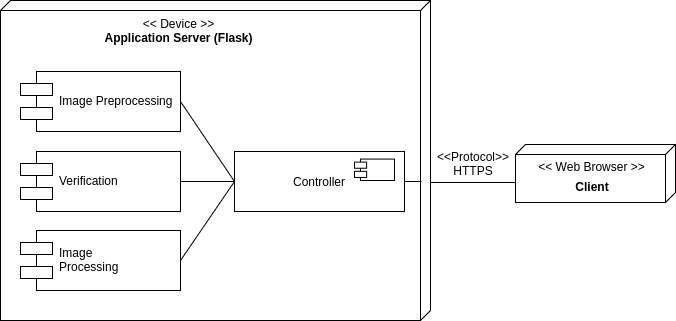
\includegraphics[scale=0.5]{img/Quant.png}
	    	\caption{Deployment Diagram}
	    \end{figure}
	    \pagebreak

\section{High Level Diagrams}

\subsection{State Diagram}
\begin{figure}[h]
	\centering
	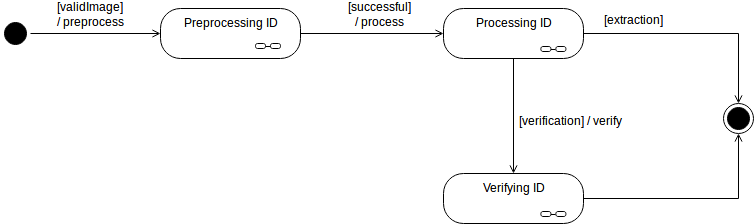
\includegraphics[scale=0.5]{img/StateModelHighLevel.png}
	\caption{High Level State Diagram}
\end{figure}
	 
\section{Services}
This section outlines the design of each individual service and in terms of UML diagrams and how services are related to one another.

\subsection{Image Processing}
The Image Processing service is the core module of the system. This service creates the image processing pipeline by applying all the necessary computer vision and processing techniques. This service is mostly used by the Extraction module to prepare the image for OCR. 
\subsubsection{Class Diagram}
The class diagram of the Image Processing module makes use of a combination of two well-known design patterns: 
\begin{itemize}
	\item \textbf{Decorator:} Different preprocessing techniques are added to the PreProcessor object at runtime.
	\item \textbf{Strategy:} Each preprocessing technique's \textit{preProcess()} algorithm can be changed at runtime.
	\begin{figure}[!h]
	    \centering
	    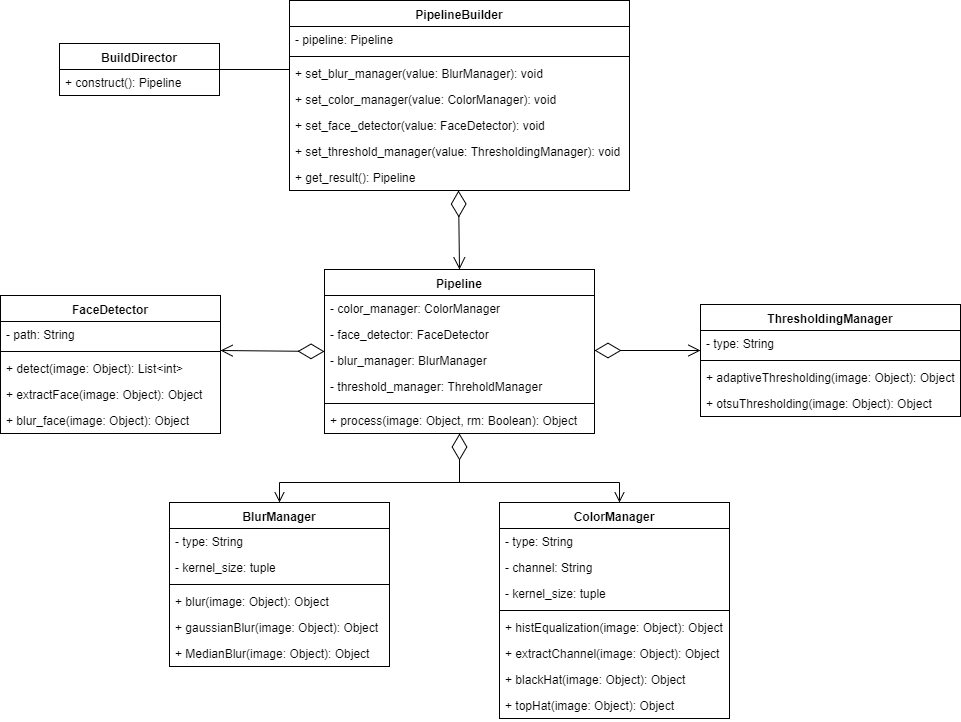
\includegraphics[scale=0.3]{img/imageProcessingClassDiagram.png}
	    \caption{Image Pre-Processing Class Diagram}
	 \end{figure}
	   \pagebreak
	 \begin{figure}[!h]
		\centering
	    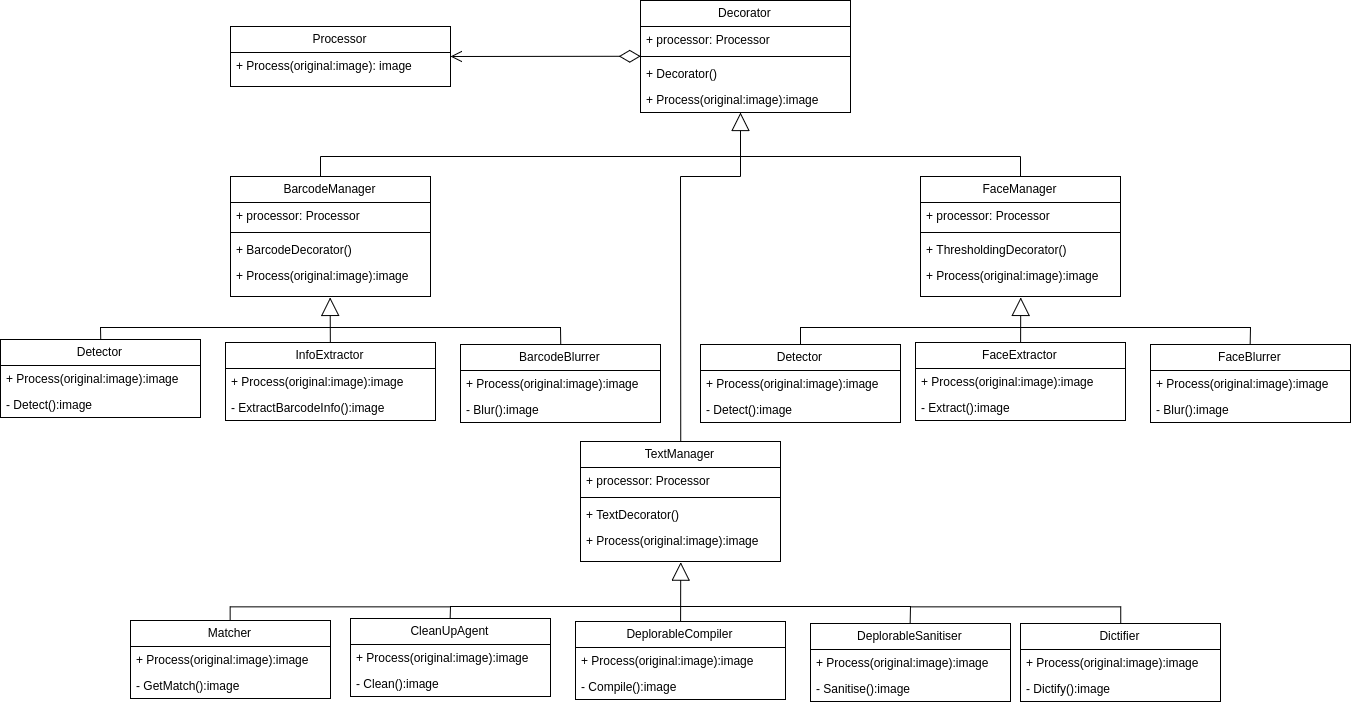
\includegraphics[scale=0.3]{img/processingClassDiagram.png}
	    \caption{Image Processing Class Diagram}
	 \end{figure}
\end{itemize}
\pagebreak
\subsubsection{Sequence Diagram}
\begin{figure}[h]
	    \centering
	    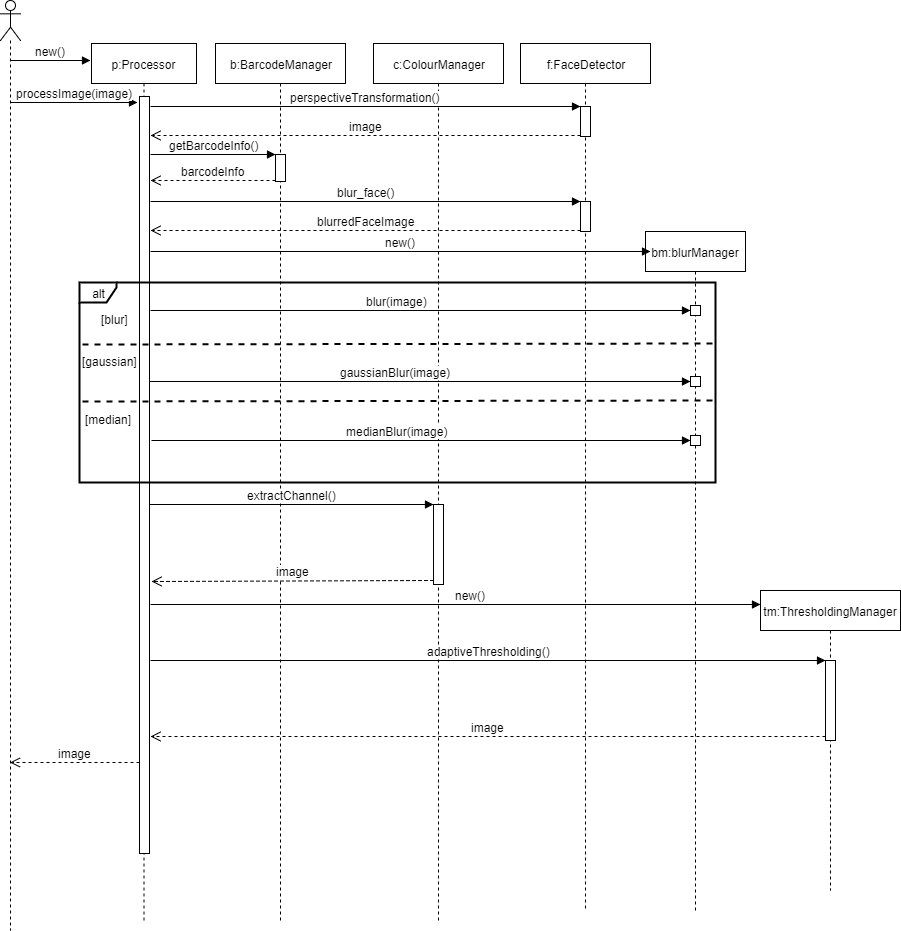
\includegraphics[scale=0.5]{img/image_processing_sequence.png}
	    \caption{Image Pre-Processing Sequence Diagram}
	 \end{figure}


\end{document}